\chapter{Realisierung und Anwendung von Softwarearchitekturen 2}
\label{ch:03_implementation-and-application-of-software-architectures_02}

\begin{universityTask}
    \begin{enumerate}[label=(\alph*)]
        \item Definieren Sie den Begriff SOA und nennen Sie vier Hauptmerkmale. Erläutern Sie zudem, was in diesem Kontext unter \q{Orchestrierung} verstanden wird.
            \universityPoints{8}
        \item Beschriften Sie die vier Elemente der nachfolgenden Abbildung eines hierarchischen Aufbaus einer SOAP-Nachricht. Erläutern Sie kurz Ihre Darstellung und Wahl.
            \begin{minipage}[t]{\textwidth}
                \begin{figure}[H]
                    \centering
                    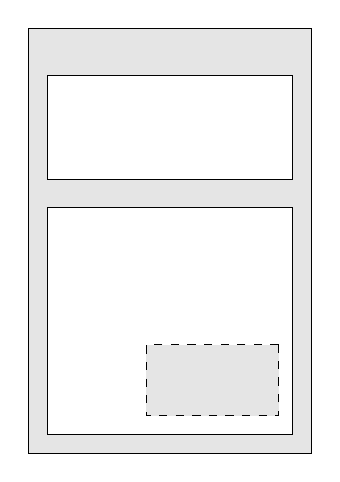
\begin{tikzpicture}[scale=0.6, transform shape,
                        box/.style={
                            draw,
                            fill=white,
                            minimum width=5.2cm,
                            font=\sffamily,
                            inner sep=8pt,
                            align=left
                        },
                        outerbox/.style={
                            draw,
                            fill=gray!20,
                            inner sep=12pt,
                            align=left,
                            font=\sffamily
                        },
                        faultbox/.style={
                            draw,
                            dashed,
                            fill=gray!20,
                            minimum width=2.8cm,
                            minimum height=1.5cm,
                            font=\sffamily,
                            inner sep=8pt,
                            align=left
                        }
                    ]

                    % Outer Envelope (solid, encompassing all)
                    \node[outerbox,
                        minimum width=6cm,
                        minimum height=9cm,
                        anchor=north west
                    ] (envelope) at (0,0) {};

                    \node[anchor=north west, font=\sffamily]
                        at ([xshift=6pt, yshift=-6pt] envelope.north west)
                        {};

                    % SOAP Header (solid, inside Envelope, top-left)
                    \node[box,
                        minimum height=2.2cm,
                        anchor=north west
                    ] (header) at ([xshift=0.4cm, yshift=-1cm] envelope.north west) {};

                    \node[anchor=north west, font=\sffamily]
                        at ([xshift=6pt, yshift=-6pt] header.north west)
                        {};

                    % SOAP Body (solid, inside Envelope, below Header)
                    \node[box,
                        minimum height=4.8cm,
                        anchor=north west
                    ] (body) at ([xshift=0.4cm, yshift=-3.8cm] envelope.north west) {};

                    \node[anchor=north west, font=\sffamily]
                        at ([xshift=6pt, yshift=-6pt] body.north west)
                        {};

                    % SOAP Fault (dashed, inside Body, bottom-right)
                    \node[faultbox,
                        anchor=south east
                    ] (fault) at ([xshift=-0.3cm, yshift=0.4cm] body.south east)
                        {};
                    \end{tikzpicture}
                \end{figure}
            \end{minipage}
            \universityPoints{4}
        \item Was versteht man unter Unternehmensarchitekturen? Definieren Sie den Begriff, nennen Sie Kernziele sowie zentrale Vorteile des Einsatzes.
            \universityPoints{6}
        \item Ordnen Sie die nachfolgend genannten Vorteile eines Enterprise Architecture Management entsprechend ihrer Wirksamkeit einem eher kurzfristigen oder eher langfristigen Zeitraum zu, und erläutern Sie die einzelnen Vorteile detailliert: \linebreak
        Unterstützung Risikoanalyse, Wertschöpfung, Entscheidungsunterstützung, Bewertung IT-Portfolio, Management Komplexität, Flexibilität, Synergiepotenzial, Capability Management, Identifikation Handlungsbedarf, Positionierung, Einschränkung Redundanz, Transparenz.
            \universityPoints{12}
    \end{enumerate}
\end{universityTask}

\section{Serviceorientierte Architektur}
\label{sec:03-01_service-oriented-architecture}

Der Text enthält die Lösung der obigen Aufgabenstellung.

\section{\ACRshort{soap}-Nachricht}
\label{sec:03-02_soap-message}

Der Text enthält die Lösung der obigen Aufgabenstellung.

\begin{minipage}[t]{\textwidth}
    \begin{figure}[H]
        \centering
        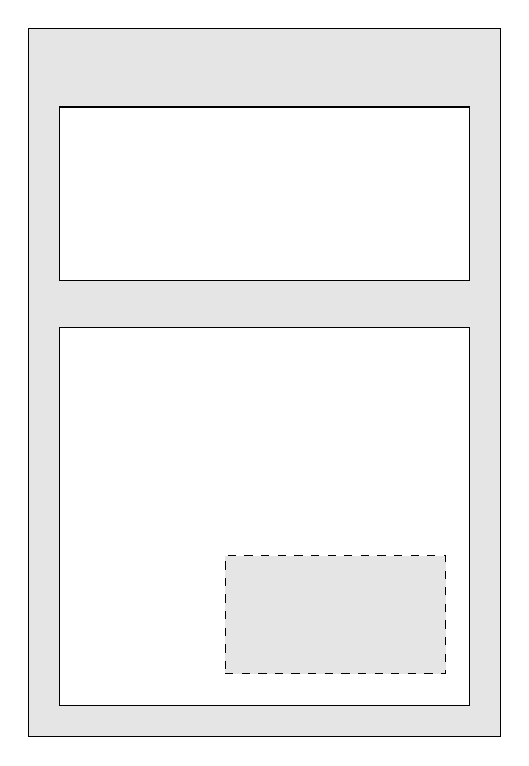
\begin{tikzpicture}[scale=1.0, transform shape,
            box/.style={
                draw,
                fill=white,
                minimum width=5.2cm,
                font=\sffamily,
                inner sep=8pt,
                align=left
            },
            outerbox/.style={
                draw,
                fill=gray!20,
                inner sep=12pt,
                align=left,
                font=\sffamily
            },
            faultbox/.style={
                draw,
                dashed,
                fill=gray!20,
                minimum width=2.8cm,
                minimum height=1.5cm,
                font=\sffamily,
                inner sep=8pt,
                align=left
            }
        ]

        % Outer Envelope (solid, encompassing all)
        \node[outerbox,
            minimum width=6cm,
            minimum height=9cm,
            anchor=north west
        ] (envelope) at (0,0) {};

        \node[anchor=north west, font=\sffamily]
            at ([xshift=6pt, yshift=-6pt] envelope.north west)
            {};

        % SOAP Header (solid, inside Envelope, top-left)
        \node[box,
            minimum height=2.2cm,
            anchor=north west
        ] (header) at ([xshift=0.4cm, yshift=-1cm] envelope.north west) {};

        \node[anchor=north west, font=\sffamily]
            at ([xshift=6pt, yshift=-6pt] header.north west)
            {};

        % SOAP Body (solid, inside Envelope, below Header)
        \node[box,
            minimum height=4.8cm,
            anchor=north west
        ] (body) at ([xshift=0.4cm, yshift=-3.8cm] envelope.north west) {};

        \node[anchor=north west, font=\sffamily]
            at ([xshift=6pt, yshift=-6pt] body.north west)
            {};

        % SOAP Fault (dashed, inside Body, bottom-right)
        \node[faultbox,
            anchor=south east
        ] (fault) at ([xshift=-0.3cm, yshift=0.4cm] body.south east)
            {};
        \end{tikzpicture}
        \caption{Hierarchischer Aufbau einer \ACRshort{soap}-Nachricht}
        \label{fig:03-02_hierarchical-structure-of-a-soap-message}
    \end{figure}
\end{minipage}

\section{Unternehmensarchitekturen}
\label{sec:03-03_enterprise-architectures}

Der Text enthält die Lösung der obigen Aufgabenstellung.

\section{Vorteile von Enterprise Architecture Management}
\label{sec:03-04_advantages-of-enterprise-architecture-management}

Der Text enthält die Lösung der obigen Aufgabenstellung.

\begin{table}[H]
    \centering
    \begin{university-table}{
        width=\textwidth,
        colspec = {X[1,c] X[3] X[5]},
    }
        Zeitraum & Vorteil & Erläuterung \\
        \SetCell[r=6]{c,m} \rotatebox{90}{\strut kurzfristig} & & \\
        & & \\
        & & \\
        & & \\
        & & \\
        & & \\
        \SetCell[r=6]{c,m} \rotatebox{90}{\strut langfristig} & & \\
        & & \\
        & & \\
        & & \\
        & & \\
        & & \\
    \end{university-table}
    \caption{Kurzfristige und langfristige Vorteile von Enterprise Architecture Management}
    \label{tab:03-04_advantages-of-enterprise-architecture-management}
\end{table}